Today there are several products either already on the market or under development that are more or less similar to Google Glass. Following is a short list (a more extensive list of devices can be found on wikipedia~\cite{ohmdWiki}) describing some of the competition Google Glass faces, with each product shown in Figure ~\ref{imagesSimilarProducts}. 

	\begin{figure}[ht!]
		\centering
    	\subfloat[Microsoft Hololens~\cite{hololens}]{{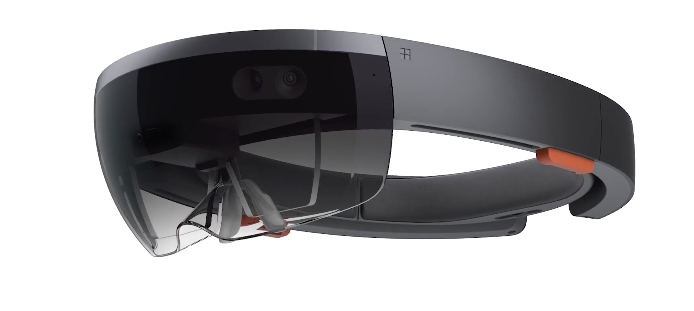
\includegraphics[width=70mm]{images/similarProducts/hololens}}}
    \qquad
    	\subfloat[Recon Jet~\cite{reconJet}]{{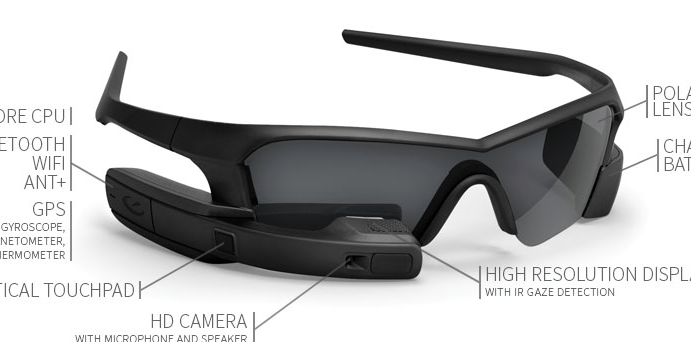
\includegraphics[width=70mm]{images/similarProducts/reconJet}}}
    \qquad
        \subfloat[GlassUp~\cite{glassUpFeatures}]{{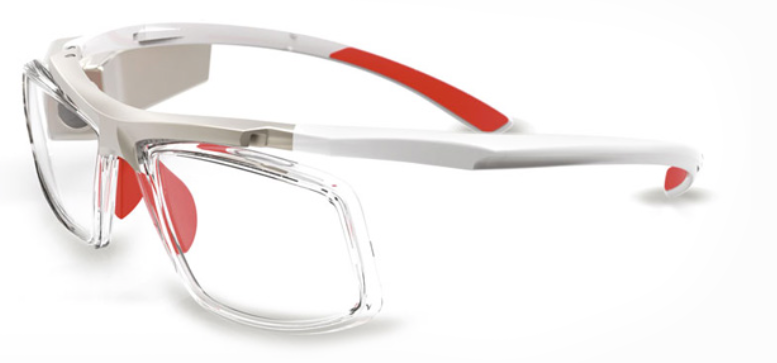
\includegraphics[width=70mm]{images/similarProducts/glassUp}}}
    \qquad
  	\subfloat[C Wear Interactive Glasses~\cite{pennyProducts}]{{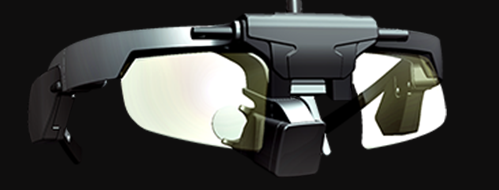
\includegraphics[width=70mm]{images/similarProducts/penny}}}
    \qquad
		\caption{There are many OHMD devices similar to Google Glass~\cite{ohmdWiki}.}
		\label{imagesSimilarProducts}
	\end{figure}
	

\begin{itemize}
\item \textbf{Microsoft Hololens}~\cite{hololens} 

Microsoft's offer in the augmented reality device space is a HUD that displays information in front of both of the user's eyes, called Microsoft Hololens, seen in Figure~\ref{imagesSimilarProducts}~(a). 
%The intention, according to Microsoft, is not to be an immediate competitor to Google Glass. Microsoft's aim is not to make the same device as Google Glass. 
However, while Google Glass is meant to be worn at all times, Microsoft Hololens is rather a device users only wear when they intend to use Microsoft Hololens. Google Glass is, as Thad Starner stated~\cite{6504855}, meant to be an extension of the self and is meant to be worn even though the user might not be actively using Google Glass at the time in order to bring helpful notifications and information to the user. Microsoft Hololens is rather a tool to be used actively for a certain purpose, such as modelling~\cite{hololensDemo}, and then put away. Google Glass may be used the same way if the user wants to, but that is not the intent.

The mot striking difference between Microsoft Hololens and Google Glass lies in the interaction with the real world. Google Glass is a two dimensional (2D) display that sits slightly above the users line of sight (see section~\ref{subsec:googleglass}). Microsoft Hololens, on the other hand, is meant to interact with the world even further.

Microsoft intends to give the user tools to work in a three dimensional (3D) space. Microsoft's concept video~\cite{hololensConceptVideo} of Microsoft Hololens shows examples of 3D modelling with the use of kinetic hand-movement detection. Microsoft Hololens will enable users to see what they are working on from different angles simply by walking around the object, just as if the object in question was real and had a physical mass.

\item \textbf{Recon Jet}~\cite{reconJet}

Recon Jet, seen in Figure~\ref{imagesSimilarProducts}~(b) is an HMD developed by Recon Instruments. Recon Jet is suited for athletes.~\cite{reconJet} Because of the target audience Recon Jet has been fitted with a display that has high contrast in order to give good readability in high ambient lighting. The display's virtual image appears as  a 30 inch wide screen at approximately 2 meters distance~\cite{reconJetSpecs}, to be compared with Google Glass' virtual image which appears as a 25 inch high definition screen seen from a distance of 2.5 meters~\cite{GlassSpecs}.

Unlike Google Glass, Recon Jet's display is located below the user's line of sight, as seen in Figure~\ref{imagesSimilarProducts}. Recon Jet's target audience, athletes, are used to having their information below line of sight. For instance a bike may have dashboard mounted to the handlebar, or an athlete might be using a watch to check the time. Google Glass is meant to be worn at all times while the location and the brightness of the display indicates that Recon Jet, however, is meant to only be used while the athlete is working out and not more regularly.

\item \textbf{GlassUp}~\cite{glassUp}

GlassUp is an Italian company that received most of its founding for the HMD device, GlassUp (seen in Figure~\ref{imagesSimilarProducts}~(c)), through the crowd-funding site Indiegogo~\cite{glassUpIndiegogo}. GlassUp has been accused of being to similar to Google Glass, partially because of the name of the device~\cite{glassUpLegal}. GlassUp does however make distinctions between the two products. On GlassUp's Indiegogo page the company made the comparison that looking at Google Glass' display was similar to looking in the back view mirror while GlassUp was similar to looking out the windscreen. The comparison referenced the fact that Google Glass' display is located above the user's line of sight, similar to a rear view mirror.

GlassUp instead displays information close to the center of the user's line of sight. GlassUp claimed, on the company's Indiegogo page, that the display was placed closer to the center of the users line of sight so that there would be less strain on the user's eyes. However, the biggest difference from Google Glass is that GlassUp is meant only to act as a second screen. GlassUp is a ``receive only'' device which displays information from the device currently connected through bluetooth, for instance a smartphone. GlassUp does not do any calculations on its own and must stay connected to a bluetooth device in order to display information~\cite{glassUpIndiegogo}.

\item \textbf{C Wear Interactive Glasses}~\cite{penny}

C Wear Interactive Glasses, seen in Figure~\ref{imagesSimilarProducts}~(d), is an industry focused device developed by Penny in V{\"a}ster{\aa}s, Sweden~\cite{pennyCompany}. C Wear Interactive Glasses projects an image onto the actual glass in front of the user's right eye and as such covers a larger area than similar devices such as Google Glass, Recon Jet and GlassUp~\cite{pennyDisplay}. The display is said to be perceived as a 75 inch display at a distance of 2.1 meters~\cite{pennyProducts}. The projection is transparent which enables users to still see what is happening in front of them.

Being industry focused C Wear Interactive Glasses is also equipped with a hands-free user interface  that does not require voice command. C Wear Interactive Glasses uses a jaw sensor which lies against the user's jawbone muscle. The sensor detects tension in the muscle, which registers as a click, to be compared with a toucn on the Google Glass touchpad~\cite{pennyProducts}.

C Wear Interactive Glasses, similar to GlassUp, is designed to be connected to an external device~\cite{pennyProducts}. However, where GlassUp is connected through bluetooth C Wear Interactive Glasses is connected through an adapter which can send data and visual information via USB and HDMI. The external device can be a smartphone, a tablet, a PC or even a TV.
\end{itemize}
%\url{http://www.microsoft.com/microsoft-hololens/en-us}
%\url{http://www.searchenginejournal.com/google-glass-alternatives/67018/}
%\url{http://www.penny.se}